\clearpage
\onecolumn

\section{Additional Experiments}
\label{appendix:additional_experiments}

\subsection{Case Study for Complete Pipeline}
\label{appendix:pipeline_case}

\begin{figure}[ht]
\centering
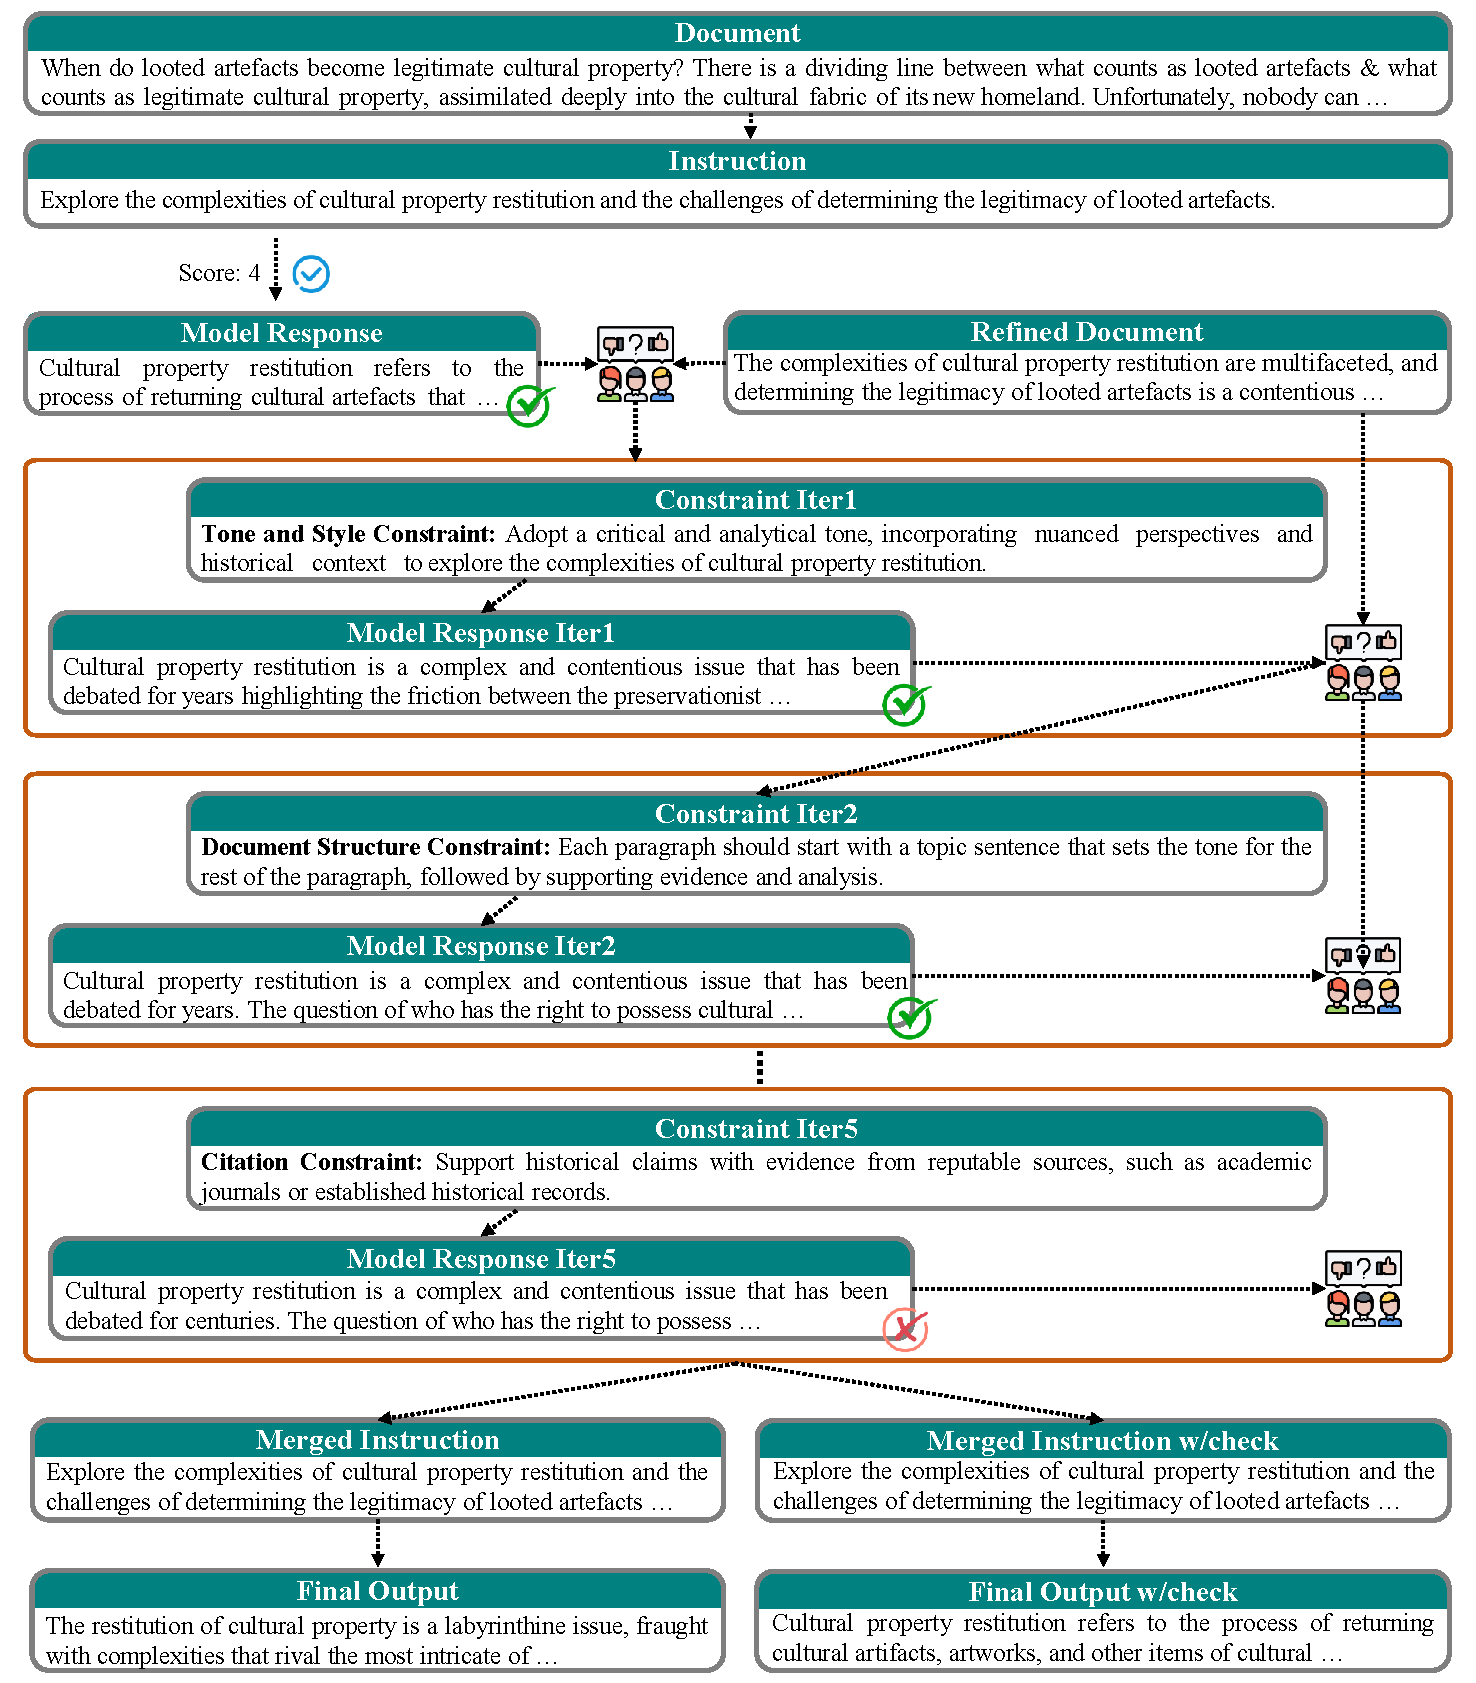
\includegraphics[width=0.75\linewidth]{source/pipeline_demo.pdf}
\caption{End-to-End Pipeline Implementation Example.}
\label{figure:appendix_pipeline_case}
\end{figure}

This section presents a detailed end-to-end demonstration of our pipeline in Figure \ref{figure:appendix_pipeline_case}. The case study provides a thorough walkthrough of each stage in our instruction generation and refinement process.

\subsection{Controlled Comparison of Instruction Synthesis Method}
\label{appendix:controlled_comparison}

Despite the superior performance reflected in Table \ref{table:main_results}, the fine-tuned results can be influenced by confounding variables. To isolate the direct impact of the instruction data quality, we conducted an additional set of experiments under a strictly controlled environment. In this setting, we re-generated datasets for all baseline methods using the identical source corpus (\textbf{Dolma v1.7}) and guidance model (\textbf{Llama-3-70B-Instruct}) employed in our DIR framework. After that, we performed SFT on the same base model with the same hyper-parameters. This ensures a direct "apples-to-apples" comparison of different instruction synthesis methods.

\begin{table}[!ht]
\centering
\caption{SFT Performance comparison under controlled experimental settings on Llama-3-8B-UltraChat. All methods are implemented with the same source document corpus (Dolma v1.7) and guidance model (Llama-3-70B-Instruct).}
\renewcommand{\arraystretch}{1.05}
\resizebox{0.9\textwidth}{!}{
\begin{tabular}{lc|ccc|cc|cc}
\toprule
\multirow{2}{*}{\textbf{Method}} & \multirow{2}{*}{\textbf{Setting}} & \multicolumn{3}{c|}{\textbf{CFBench}} & \multicolumn{2}{c|}{\textbf{FollowBench}} & \multicolumn{2}{c}{\textbf{AlpacaEval2}} \\
& & \textbf{CSR} & \textbf{ISR} & \textbf{PSR} & \textbf{HSR} & \textbf{SSR} & \textbf{LC.} & \textbf{Len} \\
\midrule
Baseline & - & 0.51 & 0.15 & 0.22 & 41.04 & 57.39 & 8.86 & 1,017 \\
Back-translation-10K & Original & $\text{0.40}_{\textcolor{deepred}{\text{-0.11}}}$ & $\text{0.11}_{\textcolor{deepred}{\text{-0.04}}}$ & $\text{0.15}_{\textcolor{deepred}{\text{-0.07}}}$ & $\text{21.19}_{\textcolor{deepred}{\text{-19.85}}}$ & $\text{33.92}_{\textcolor{deepred}{\text{-23.47}}}$ & $\text{0.96}_{\textcolor{deepred}{\text{-7.90}}}$ & 2,966 \\
Back-and-forth-10K & Original & $\text{0.58}_{\textcolor{deepgreen}{\text{+0.07}}}$ & $\text{0.20}_{\textcolor{deepgreen}{\text{+0.05}}}$ & $\text{0.27}_{\textcolor{deepgreen}{\text{+0.05}}}$ & $\text{44.65}_{\textcolor{deepgreen}{\text{+3.61}}}$ & $\text{61.58}_{\textcolor{deepgreen}{\text{+4.19}}}$ & $\text{10.06}_{\textcolor{deepgreen}{\text{+1.20}}}$ & 1,440 \\
ShareGPT-10K & Re-run & $\text{0.59}_{\textcolor{deepgreen}{\text{+0.08}}}$ & $\text{0.20}_{\textcolor{deepgreen}{\text{+0.05}}}$ & $\text{0.31}_{\textcolor{deepgreen}{\text{+0.09}}}$ & $\text{44.50}_{\textcolor{deepgreen}{\text{+3.46}}}$ & $\text{59.20}_{\textcolor{deepgreen}{\text{+1.81}}}$ & $\text{12.70}_{\textcolor{deepgreen}{\text{+3.84}}}$ & 1,570 \\
Self-Instruct-10K & Re-run & $\text{0.42}_{\textcolor{deepred}{\text{-0.09}}}$ & $\text{0.11}_{\textcolor{deepred}{\text{-0.04}}}$ & $\text{0.16}_{\textcolor{deepred}{\text{-0.06}}}$ & $\text{15.00}_{\textcolor{deepred}{\text{-26.04}}}$ & $\text{32.00}_{\textcolor{deepred}{\text{-25.39}}}$ & $\text{8.50}_{\textcolor{deepred}{\text{-0.36}}}$ & 2,384 \\
Evol-Instruct-10K & Re-run & $\text{0.55}_{\textcolor{deepgreen}{\text{+0.04}}}$ & $\text{0.21}_{\textcolor{deepgreen}{\text{+0.06}}}$ & $\text{0.26}_{\textcolor{deepgreen}{\text{+0.04}}}$ & $\text{45.20}_{\textcolor{deepgreen}{\text{+4.16}}}$ & $\text{59.80}_{\textcolor{deepgreen}{\text{+2.41}}}$ & $\text{8.80}_{\textcolor{deepred}{\text{-0.06}}}$ & 890 \\
MUFFIN-10K & Re-run & $\text{0.48}_{\textcolor{deepred}{\text{-0.03}}}$ & $\text{0.15}_{\textcolor{deepgreen}{\text{+0.00}}}$ & $\text{0.20}_{\textcolor{deepred}{\text{-0.02}}}$ & $\text{29.50}_{\textcolor{deepred}{\text{-11.54}}}$ & $\text{46.20}_{\textcolor{deepred}{\text{-11.19}}}$ & $\text{4.01}_{\textcolor{deepred}{\text{-4.85}}}$ & 990 \\
Conifer-10K & Re-run & $\text{0.52}_{\textcolor{deepgreen}{\text{+0.01}}}$ & $\text{0.18}_{\textcolor{deepgreen}{\text{+0.03}}}$ & $\text{0.23}_{\textcolor{deepgreen}{\text{+0.01}}}$ & $\text{43.20}_{\textcolor{deepgreen}{\text{+2.16}}}$ & $\text{58.50}_{\textcolor{deepgreen}{\text{+1.11}}}$ & $\text{11.50}_{\textcolor{deepgreen}{\text{+2.64}}}$ & 850 \\
I-SHEEP-10K & Re-run & $\text{0.55}_{\textcolor{deepgreen}{\text{+0.04}}}$ & $\text{0.18}_{\textcolor{deepgreen}{\text{+0.03}}}$ & $\text{0.25}_{\textcolor{deepgreen}{\text{+0.03}}}$ & $\text{36.00}_{\textcolor{deepred}{\text{-5.04}}}$ & $\text{52.50}_{\textcolor{deepred}{\text{-4.89}}}$ & $\text{7.20}_{\textcolor{deepred}{\text{-1.66}}}$ & 1,070 \\
Suri-10K & Re-run & $\text{0.53}_{\textcolor{deepgreen}{\text{+0.02}}}$ & $\text{0.17}_{\textcolor{deepgreen}{\text{+0.02}}}$ & $\text{0.23}_{\textcolor{deepgreen}{\text{+0.01}}}$ & $\text{43.00}_{\textcolor{deepgreen}{\text{+1.96}}}$ & $\text{58.08}_{\textcolor{deepgreen}{\text{+0.69}}}$ & $\text{9.50}_{\textcolor{deepgreen}{\text{+0.64}}}$ & 1,980 \\
Crab-10K & Re-run & $\text{0.54}_{\textcolor{deepgreen}{\text{+0.03}}}$ & $\text{0.17}_{\textcolor{deepgreen}{\text{+0.02}}}$ & $\text{0.23}_{\textcolor{deepgreen}{\text{+0.01}}}$ & $\text{38.50}_{\textcolor{deepred}{\text{-2.54}}}$ & $\text{55.50}_{\textcolor{deepred}{\text{-1.89}}}$ & $\text{8.80}_{\textcolor{deepred}{\text{-0.06}}}$ & 1,105 \\
\textbf{DIR-10K} & Re-run & \textbf{$\text{0.61}_{\textcolor{deepgreen}{\text{+0.10}}}$} & \textbf{$\text{0.24}_{\textcolor{deepgreen}{\text{+0.09}}}$} & \textbf{$\text{0.31}_{\textcolor{deepgreen}{\text{+0.09}}}$} & \textbf{$\text{50.69}_{\textcolor{deepgreen}{\text{+9.65}}}$} & \textbf{$\text{63.89}_{\textcolor{deepgreen}{\text{+6.50}}}$} & \textbf{$\text{21.00}_{\textcolor{deepgreen}{\text{+12.14}}}$} & 1,813 \\
\bottomrule
\end{tabular}}
\label{table:controlled_comparison}
\end{table}

As shown in Table \ref{table:controlled_comparison}, DIR-10K consistently outperforms other synthesis methods across both complex and general instruction benchmarks under controlled conditions. This confirms that the observed gains on instruction following are attributable to the data synthesis method rather than the initial choice of data or models. Notably, the results also reveal the sensitivity of different methods to initial configurations: while Self-Instruct and Suri scaled effectively with our source corpus, other methods such as Conifer and Crab showed diminished performance, suggesting their original performance may have benefited from specific private data distributions.

Meanwhile, robust methods like Evol-Instruct and ShareGPT performed comparably, suggesting their original configurations were already strong.

In summary, this controlled analysis provides stronger evidence for the effectiveness of the DIR framework, demonstrating that its advantages are attributable to the methodology itself rather than the initial choice of data or models.

\subsection{Impact on Fundamental Capabilities}

Previous methods have indicated LLMs may suffer from capability degradation during preference alignment phase, which is also known as alignment tax ~\cite{ouyang2022training}. To evaluate this concern, we tested our DIR method on several fundamental capability benchmarks: 1) World Knowledge: MMLU \cite{hendrycks2021measuring}; 2) Commonsense Reasoning: CommonsenseQA (CQA) \cite{talmor-etal-2019-commonsenseqa} and Natural Questions (NQ) \cite{kwiatkowski2019natural}; 3) Coding: HumanEval \cite{chen2021evaluatinglargelanguagemodels}; and 4) Mathematics: GSM8K \cite{cobbe2021trainingverifierssolvemath}.

\begin{table}[!ht]
\centering
\caption{Evaluation results of fundamental capabilities of models optimized by DIR.}
\renewcommand{\arraystretch}{0.95}
\resizebox{0.8\textwidth}{!}{
\begin{tabular}{l|l|ccccc|c}
\toprule
\textbf{Base Model} & \textbf{Method} & \textbf{MMLU} & \textbf{CQA} & \textbf{NQ} & \textbf{HumanEval} & \textbf{GSM8K} & \textbf{AVG} \\
\midrule
\multirow{3}{*}{Llama-3-8B-UltraChat}
& Baseline & 64.00 & 72.97 & 29.61 & 30.49 & 57.47 & 50.90 \\
& DIR-SFT & 61.64 & 73.63 & 30.54 & 29.88 & 54.59 & 50.05 \\
& DIR-RL & 63.48 & 74.15 & 31.27 & 29.53 & 58.29 & \textbf{51.34} \\
\midrule
\multirow{2}{*}{Qwen-2.5-7B-UltraChat}
& Baseline & 73.64 & 82.39 & 25.68 & 52.20 & 81.65 & 63.11 \\
& DIR-SFT & 73.35 & 82.56 & 25.76 & 55.49 & 84.38 & 64.30 \\
& DIR-RL & 73.51 & 83.42 & 25.23 & 56.68 & 85.51 & \textbf{64.87} \\
\midrule
\multirow{2}{*}{Llama-3-8B-Tulu}
& Baseline & 65.43 & 79.44 & 32.22 & 50.61 & 64.14 & 58.36 \\
& DIR-SFT & 64.95 & 79.92 & 34.62 & 50.85 & 63.70 & \textbf{58.80} \\
& DIR-RL & 64.27 & 79.13 & 31.56 & 51.18 & 63.41 & 57.91  \\
\bottomrule
\end{tabular}}
\label{table:fundamental}
\end{table}

As shown in Table \ref{table:fundamental}, our method does not have a negative impact on fundamental capabilities. Specifically, DIR-RL improves the average performance of Llama-3-8B-UltraChat and Qwen-2.5-7B-UltraChat by 0.44 and 1.76 points, respectively. Similarly, DIR-SFT shows improvements on Qwen-2.5-7B-UltraChat and Llama-3-8B-Tulu by 1.19 and 0.44 points. This indicates that instructions synthesized from documents with evenly sampled distributions also exhibit even distribution, which is helpful for maintaining the fundamental knowledge and capabilities acquired during pre-train stage.

% \subsection{Robustness to Document Quality}

% \begin{table}[!ht]
% \centering
% \caption{Comparison of model performance when fine-tuned on instructions from different document sets.}
% \renewcommand{\arraystretch}{1.0}
% \resizebox{0.48\textwidth}{!}{
% \begin{tabular}{c|ccc|cc|cc}
% \toprule
% \multirow{2}{*}{\textbf{Data}} & \multicolumn{3}{c|}{\textbf{CFBench}} & \multicolumn{2}{c|}{\textbf{FollowBench}} & \multicolumn{2}{c}{\textbf{AlpacaEval2}} \\
% & \textbf{CSR} & \textbf{ISR} & \textbf{PSR} & \textbf{HSR} & \textbf{SSR} & \textbf{LC.} & \textbf{Len} \\
% \midrule
% random 1k & 0.61	& 0.23	& 0.33	& 45.85	& 60.21	& 17.15	& 1,611 \\
% low-quality 1k	& 0.60	& 0.22	& 0.30	& 44.00	& 59.83	& 16.10	& 1,685 \\
% \bottomrule
% \end{tabular}}
% \label{table:Robustness}
% \end{table}

% As discussed in Section \ref{sec:IIR}, our framework primarily utilizes documents to extract constraints rather than as direct fine-tuning targets. During fine-tuning, we use outputs from the guidance model as targets, which insulates the process from document quality issues. Moreover, we implemented multiple safeguards in our data production pipeline, which provides inherent robustness against document noise.

% To empirically validate our method's robustness to document quality, we conducted an additional experiment comparing two document sets: (1) a "low-quality" subset comprising the 1,000 lowest-scoring documents from DIR-10k (evaluated by GPT-4 across helpfulness, completeness, and harmlessness dimensions), and (2) a randomly sampled set of 1,000 documents from the same corpus.

% Table \ref{table:Robustness} presents the performance comparison of Llama-3-8B-UltraChat models fine-tuned on instructions derived from these two document sets. The results demonstrate negligible performance differences across all evaluation benchmarks. This empirical evidence confirms that our method maintains consistent performance regardless of input document quality, validating its robustness.

% Additionally, we provide the number of samples at each stage of the iterative process. As shown in Table \ref{table:Efficiency}, despite starting with a large number of initial documents, only 15\% of them are retained for iterative instruction refinement. Furthermore, nearly 50\% of the documents are filtered out during the iterations, leaving only the highest-quality samples for final training. This demonstrates how our carefully designed strategies effectively maintain sample quality across multiple iterations.

% \begin{table}[!ht]
% \centering
% \caption{Progressive reduction in sample size through filtering stages and five iterations.}
% \renewcommand{\arraystretch}{0.95}
% \resizebox{0.4\textwidth}{!}{
% \begin{tabular}{c|c}
% \toprule
% \textbf{Stage} & \textbf{Sample Number}\\
% \midrule
% Rule-based Filtering & 300k \\
% Density-based Sampling	& 60k \\
% Instruction Scoring	& 20k \\
% Iteration 1	& 17.3k \\
% Iteration 2	& 15.2k \\
% Iteration 3	& 13.7k \\
% Iteration 4	& 12.7k \\
% Iteration 5	& 11.9k \\
% \bottomrule
% \end{tabular}}
% \label{table:Efficiency}
% \end{table}

\subsection{Influence of Guidance Model Size}
\label{sec:Guidance_Model_Size}

\begin{table}[!ht]
\centering
\caption{Experiment results on Qwen-2.5-7B-UltraChat fine-tuned with different guidance model size.}
\renewcommand{\arraystretch}{0.95}
\resizebox{0.4\textwidth}{!}{
\begin{tabular}{c|cc|cc}
\toprule
\multirow{2}{*}{\textbf{Guid. Model}} & \multicolumn{2}{c}{\textbf{FollowBench}} & \multicolumn{2}{c}{\textbf{AlpacaEval2}} \\
& \textbf{HSR}   & \textbf{SSR}   & \textbf{LC.}      & \textbf{Len}  \\
\midrule
\begin{tabular}[c]{@{}c@{}}Baseline\end{tabular}  & 47.71    & 64.79  & 10.87   & 836   \\
\midrule
14B     & 57.72   & 70.59   & 29.13   & 1,501   \\
32B     & \textbf{60.06}   & \textbf{71.97}   & 26.39   & 1,309    \\
72B     & 59.07   & 71.35   & \textbf{32.43}  & 1,779     \\
\bottomrule
\end{tabular}}
\label{table:guidance_size}
\end{table}

In Table \ref{table:guidance_size}, we investigate the impact of guidance model size on DIR's performance. We performed experiments with Qwen-2.5-7B-UltraChat as the base model, while varying the guidance model size from 14B to 72B parameters. As shown, all guidance models with different sizes significantly improve instruction-following ability compared to the baseline, while larger models generally provide greater improvement. On the other hand, even the 14B guidance model demonstrates remarkable improvement. This scalability across different model sizes highlights the robustness and efficiency of our proposed approach.

These findings suggest that DIR's effectiveness is not strictly dependent on large guidance models. The method effectively leverages both document knowledge and model knowledge through judging mechanism to generate meaningful constraints, making it practical and efficient even with relatively smaller guidance models.

\section{Implementation Details}
\label{appendix:additional_details}

\subsection{Model Training Hyper-parameters}
\label{appendix:hyper-parameters}

This section details our model training configuration. We employed Supervised Fine-Tuning (SFT) based on the LlamaFactory \cite{zheng2024llamafactory} framework, with hyper-parameters as outlined in Table \ref{table:hyperparams}. Furthermore, we conducted Reinforcement Learning (RL) experiments using the verl \cite{verl} framework, and the corresponding hyper-parameters are listed in Table \ref{tab:hyperparams_rl}.

\begin{table}[!ht]
\centering
\renewcommand{\arraystretch}{1.1}
\caption{Hyper-parameters for SFT experiments.}
\resizebox{0.45\textwidth}{!}{
\begin{tabular}{l|cc}
\toprule
\textbf{Configuration} & \textbf{Llama-3-8B}   & \textbf{Qwen-2.5-7B}   \\
\midrule
Max Sequence Length    & 4096                  & 4096                   \\
Learning Rate          & 1e-5                  & 1e-5                   \\
LR Scheduler           & cosine decay          & cosine decay           \\
Training Epochs        & 3                     & 3                      \\
Batch Size             & 64                    & 64                     \\
Mixed Precision        & bf16                  & bf16                   \\
DeepSpeed ZeRO Stage   & stage 2               & stage 2                \\
\bottomrule
\end{tabular}}
\label{table:hyperparams}
\end{table}

\begin{table*}[!ht]
\centering
\renewcommand{\arraystretch}{1.1}
\caption{Hyper-parameters for RL experiments.}
\resizebox{0.50\linewidth}{!}{
\begin{tabular}{lccc}
\toprule
\textbf{Configuration} & \textbf{GRPO} & \textbf{PPO} & \textbf{Reinforce++} \\
\midrule
Generation Batch Size           & 512      & 256      & 256 \\
Training Batch Size             & 256      & 256      & 256 \\
Max Prompt Length               & 1024     & 1024     & 1024 \\
Max Response Length             & 4096     & 4096     & 4096 \\
Actor Learning Rate             & 3e-6     & 3e-6     & 3e-6 \\
Actor Mini Batch Size           & 64       & 64       & 64 \\
Actor Micro Batch Size          & 8        & 8        & 8 \\
Use KL Loss                     & False    & True     & True \\
KL Loss Coefficient             & 0.0      & 0.001    & 0.001 \\
Rollout Log Prob Batch Size     & 16       & 16       & 16 \\
Rollout Number ($N$)            & 8        & --       & 8 \\
Ref Log Prob Batch Size         & 16       & 16       & 16 \\
Critic Learning Rate            & --       & 1e-5     & -- \\
Critic Micro Batch Size         & --       & 8        & -- \\
GPUs Per Node                   & 8        & 8        & 8 \\
Number of Nodes                 & 2        & 2        & 2 \\
Total Epochs                    & 10       & 10       & 10 \\
\bottomrule
\end{tabular}
}
\label{tab:hyperparams_rl}
\end{table*}

\subsection{Prompt Templates}
\label{appendix:prompt_templates}

This section presents the prompts used in our data generation pipeline. For Initial Instruction Generation, the prompts serve different purposes from initial instruction generation through back-translation (Figure~\ref{figure:prompt_back_ins}) to document refining (Figure~\ref{figure:prompt_document_polish}) and instruction scoring (Figure~\ref{figure:prompt_ins_score}). For Iterative Instruction Refinement, the prompts serve different purposes from constraint generation (Figure~\ref{figure:cons_generate}), constraint verification (Figure~\ref{figure:cons_check}), and finally combines all elements into refined instructions (Figure~\ref{figure:cons_combine}).

\subsection{Instruction Score Criteria}
\label{appendix:ins_score_case}

This section presents the detailed score criteria of the instruction quality through representative examples. As illustrated in Figure~\ref{figure:ins_score_case_show}, we provide a diverse set of instructions spanning the entire quality spectrum (scores 1-5). Each score category is exemplified by five carefully selected cases, where score 1 represents basic quality and score 5 demonstrates exceptional quality.

\begin{figure}[ht]
\centering
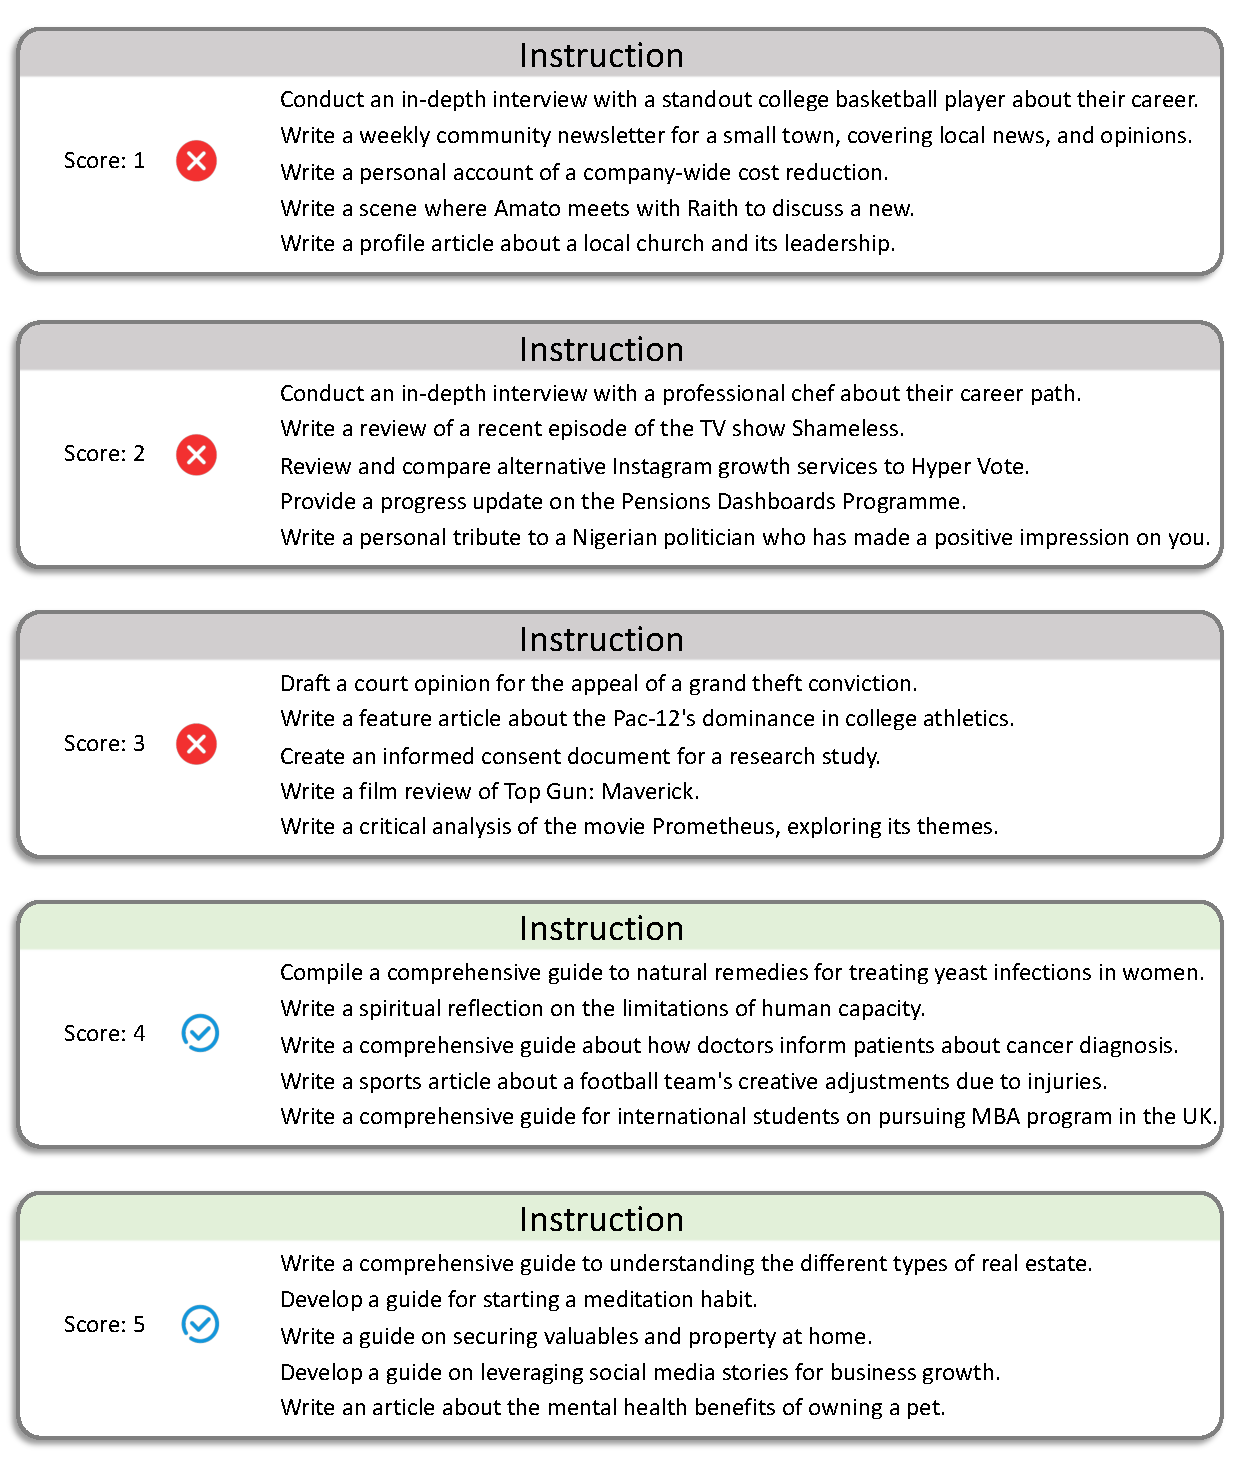
\includegraphics[width=0.75\linewidth]{source/prompt/ins_score_case.pdf}
\caption{Examples of instructions at different score levels (1-5), where each score level is illustrated with five representative cases. Score 1 represents the lowest quality while score 5 represents the highest quality.}
\label{figure:ins_score_case_show}
\end{figure}


\begin{figure}[ht]
\centering
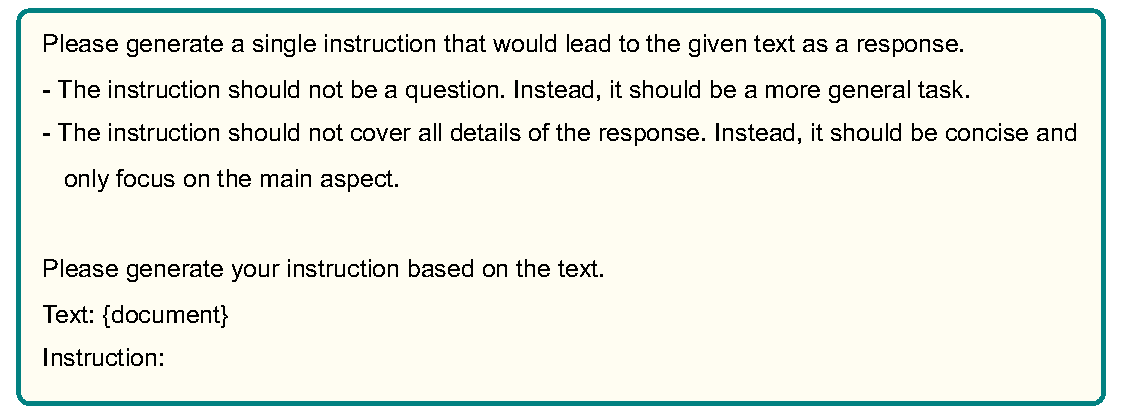
\includegraphics[width=0.8\linewidth]{source/prompt/prompt_back_ins.pdf}
\caption{Prompt for generating initial instructions through back-translation.}
\label{figure:prompt_back_ins}
\end{figure}

\begin{figure}[ht]
\centering
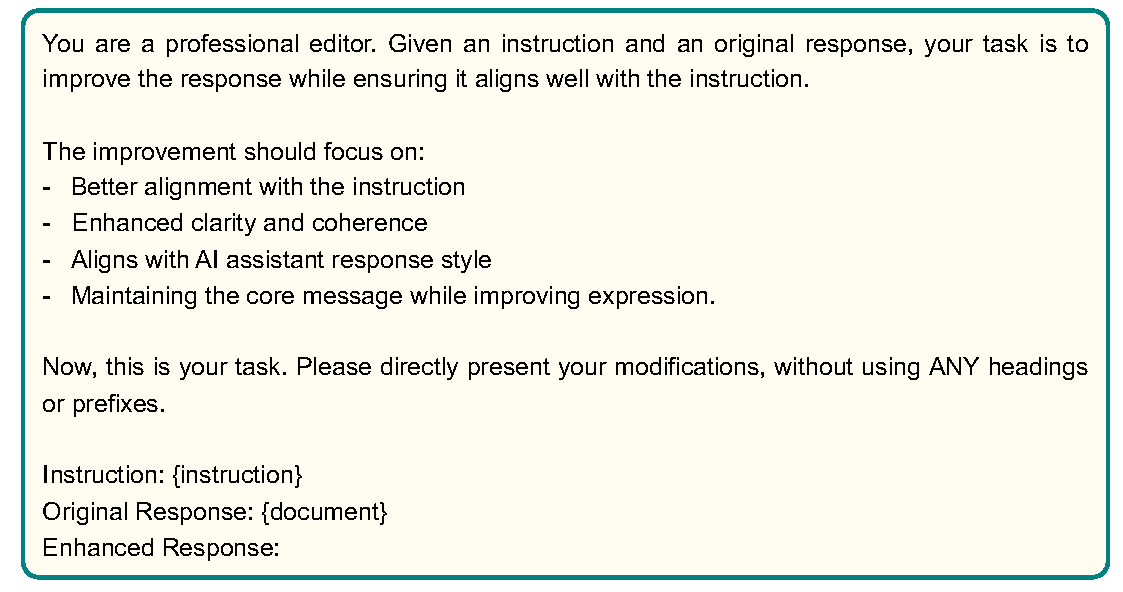
\includegraphics[width=0.8\linewidth]{source/prompt/prompt_document_polish.pdf}
\caption{Prompt for refining document content.}
\label{figure:prompt_document_polish}
\end{figure}

\begin{figure}[ht]
\centering
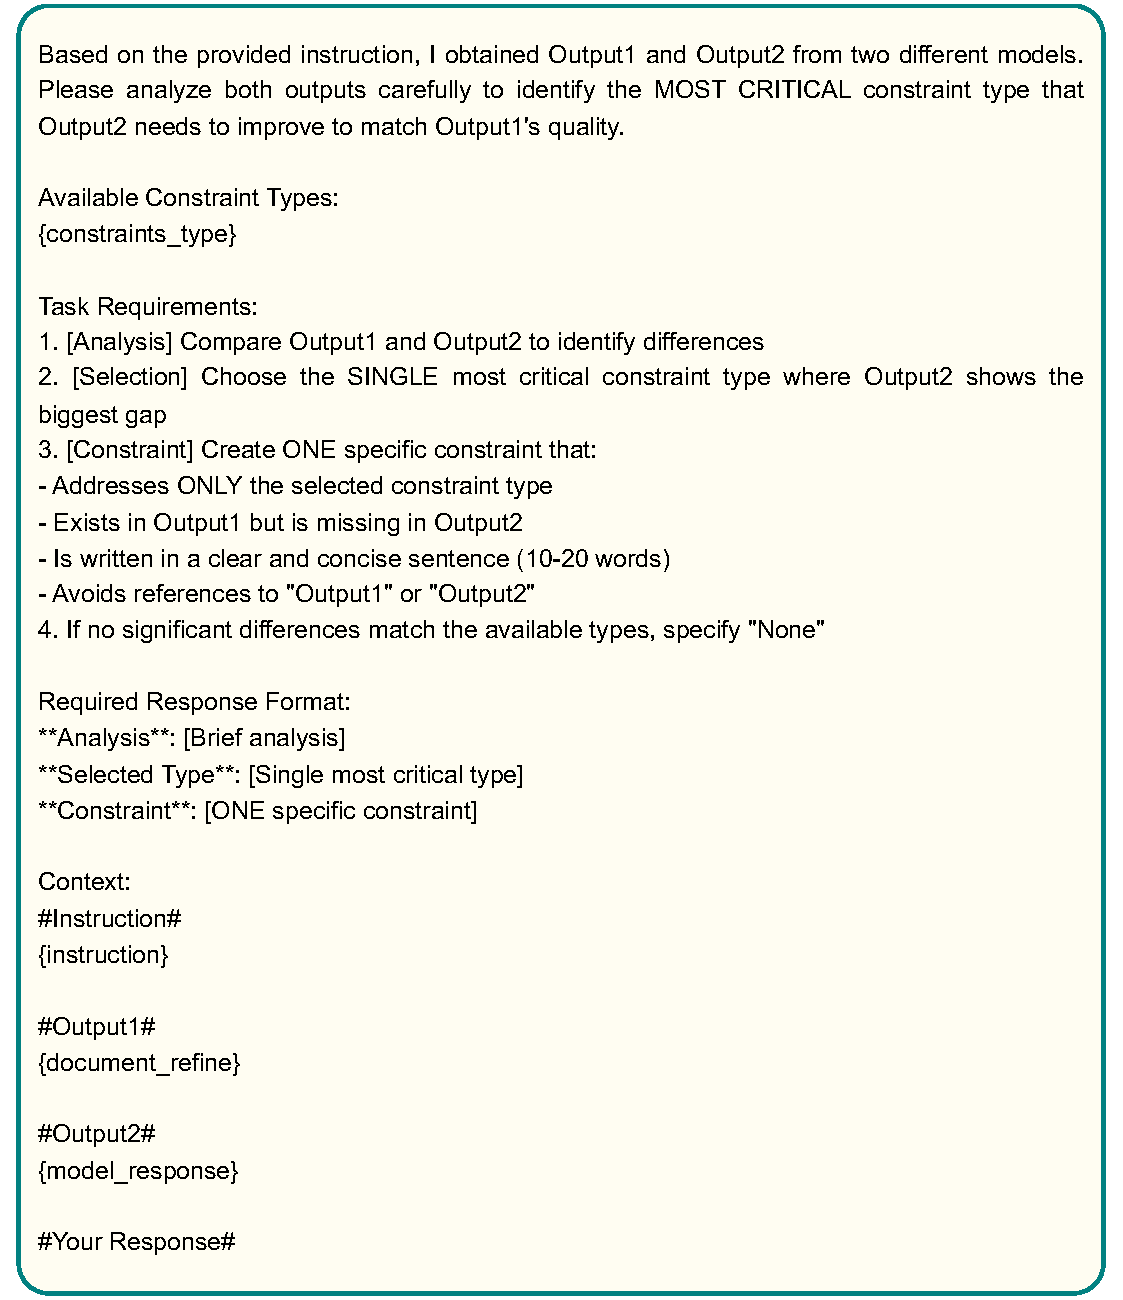
\includegraphics[width=0.8\linewidth]{source/prompt/cons_generate.pdf}
\caption{Prompt for generating constraints based on judge.}
\label{figure:cons_generate}
\end{figure}

\begin{figure}[ht]
\centering
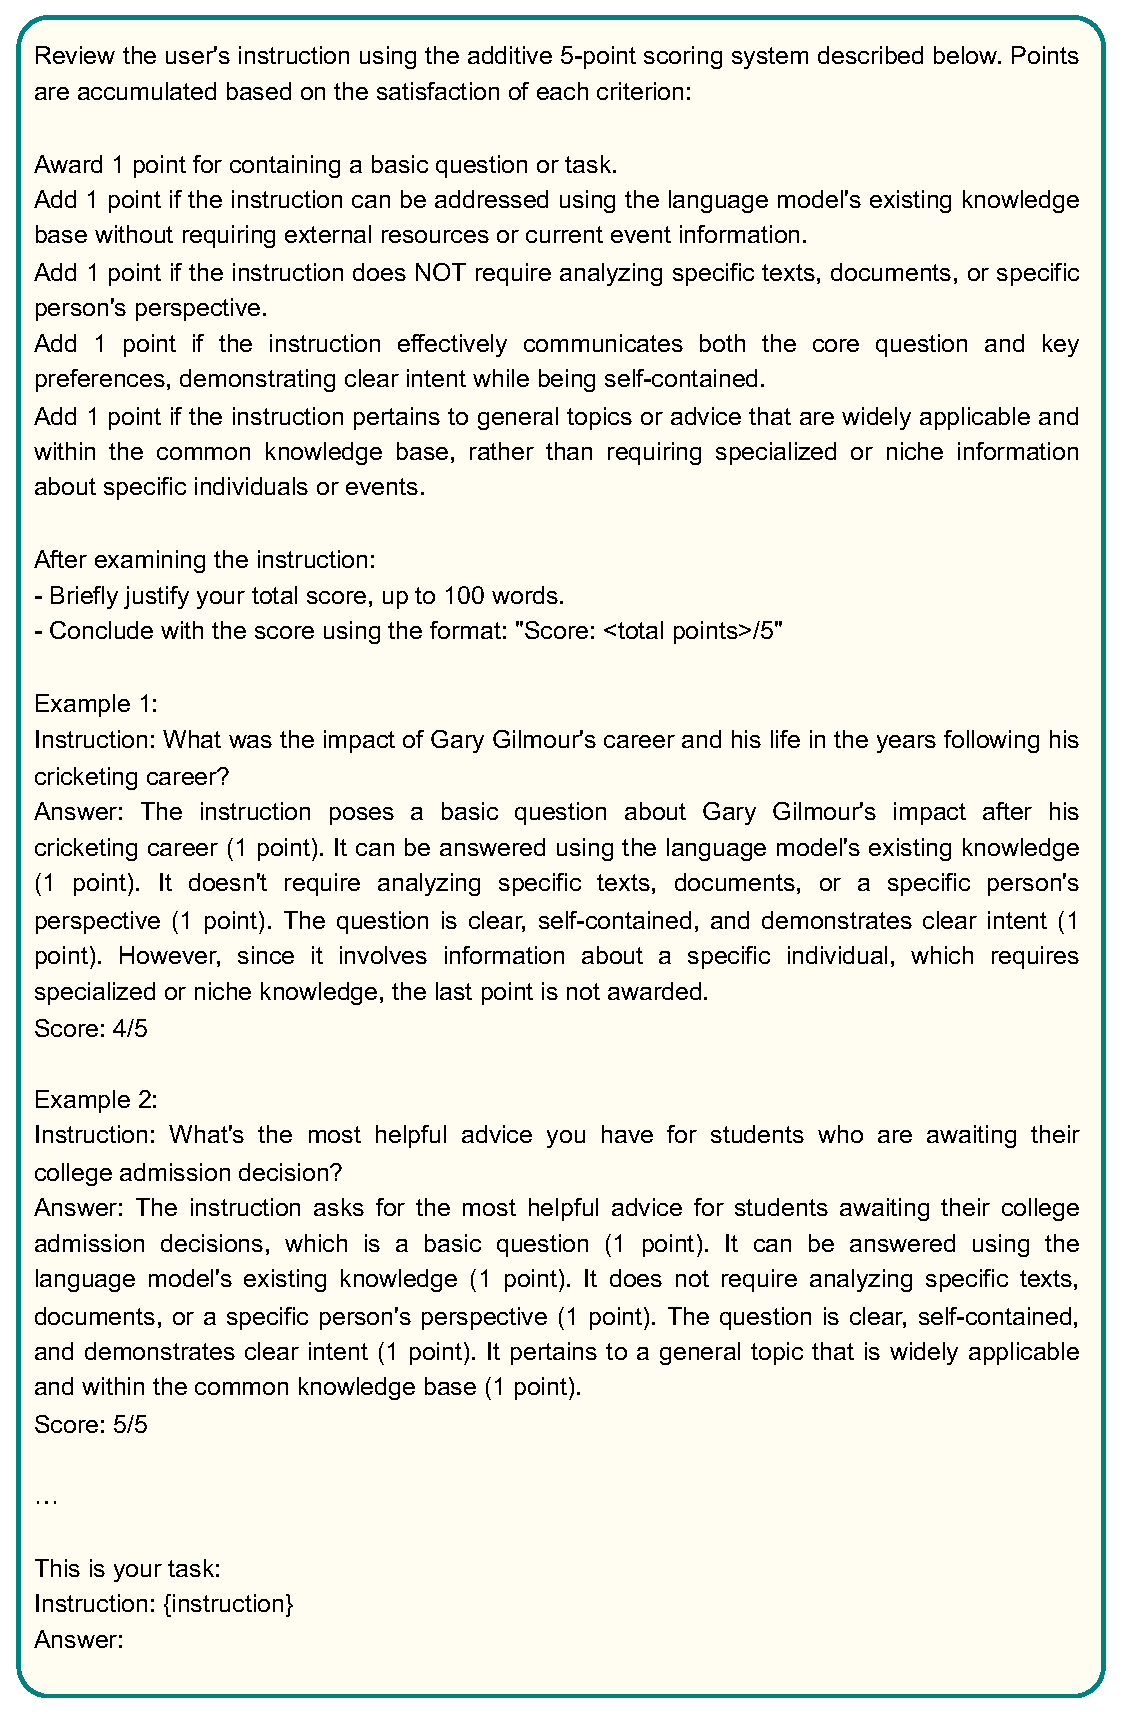
\includegraphics[width=0.8\linewidth]{source/prompt/prompt_ins_score.pdf}
\caption{Prompt for scoring initial instructions.}
\label{figure:prompt_ins_score}
\end{figure}

\begin{figure}[ht]
\centering
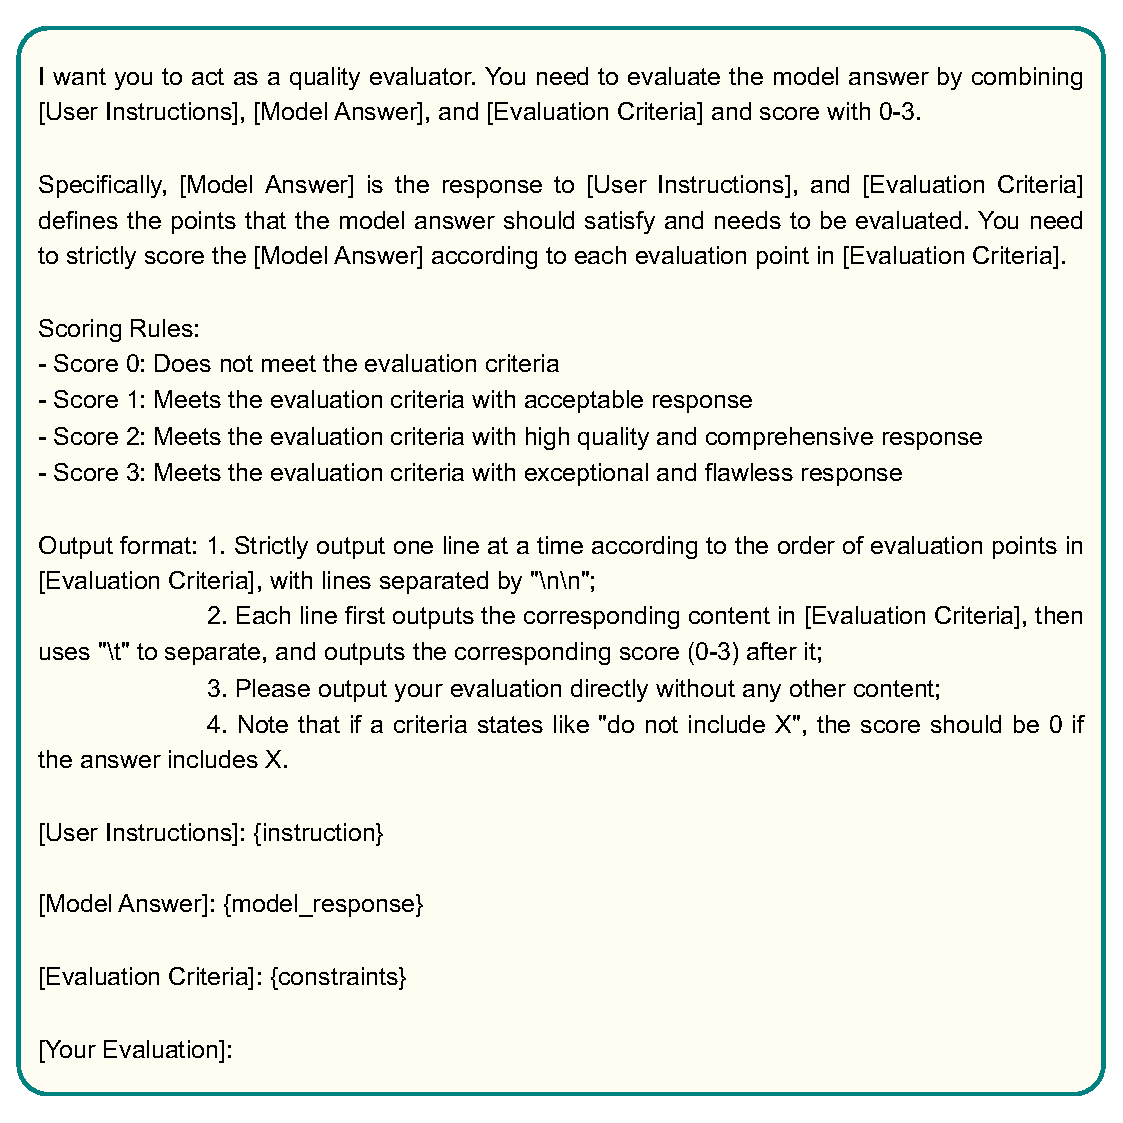
\includegraphics[width=0.8\linewidth]{source/prompt/cons_check.pdf}
\caption{Prompt for verifying model responses against constraints.}
\label{figure:cons_check}
\end{figure}

\begin{figure}[ht]
\centering
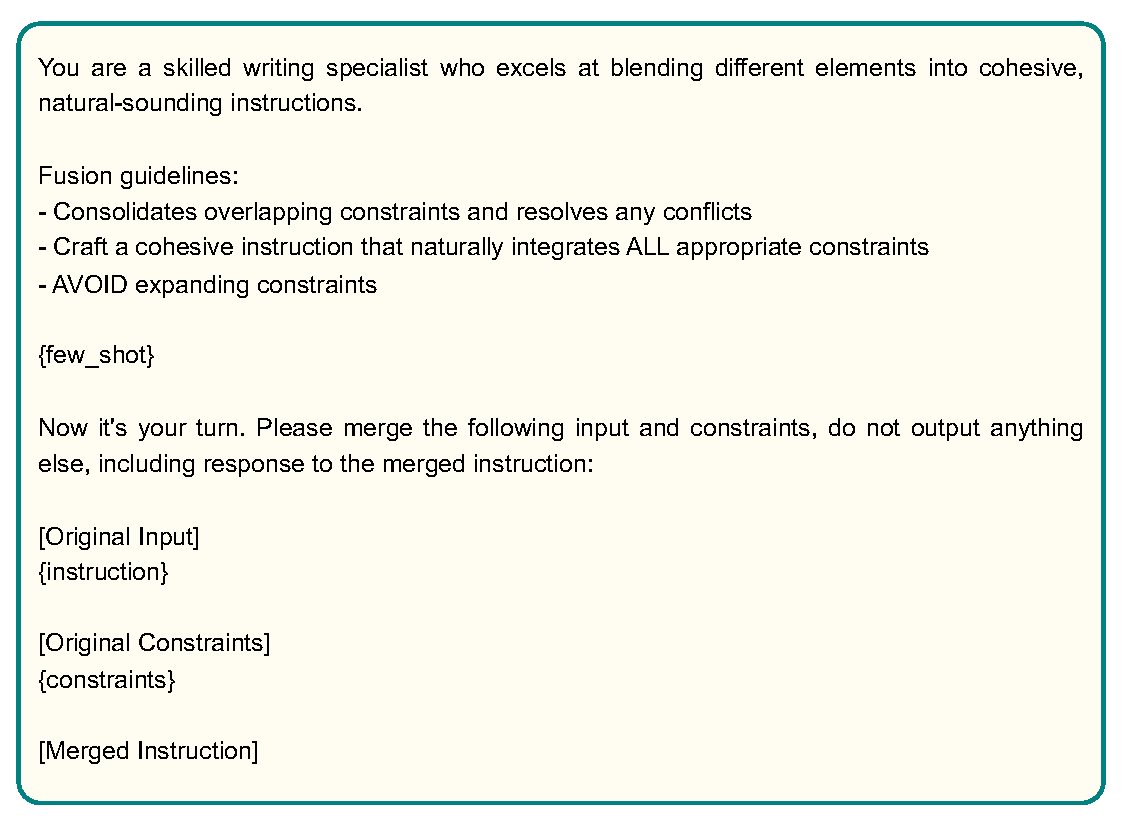
\includegraphics[width=0.8\linewidth]{source/prompt/cons_combine.pdf}
\caption{Prompt for combining instructions with constraints.}
\label{figure:cons_combine}
\end{figure}

